%!TeX TXS-program:bibliography = txs:///biber

\documentclass[letterpaper,man,biblatex]{apa6}

\usepackage[style=apa,backend=biber]{biblatex}
\addbibresource{zotero-crps.bib}

\usepackage[american]{babel}
\DeclareLanguageMapping{american}{american-apa}
\usepackage[utf8]{inputenc}
\usepackage{csquotes}
\usepackage{amsmath}
\usepackage{graphicx}
\usepackage{etoolbox}
\usepackage{geometry}
\usepackage[usenames,dvipsnames]{xcolor}
\usepackage{versions}
\newcommand{\red}{\color{red}}
\newcommand{\blue}{\color{blue}}
\newcommand{\green}{\color{green}}

%%% 
%%%   INSTRUCTIONS
%%%
%%% Just comment out one or the other of the "togglefalse/toggletrue" pairs

\newtoggle{final}
\newtoggle{blind}
\togglefalse{final}
%\toggletrue{final}
%\toggletrue{blind}
\togglefalse{blind}

% 
% Align numbers in tables
%

\usepackage{dcolumn}
\newcolumntype{d}[1]{D{.}{.}{#1}}
\usepackage{siunitx}
%
% Include/exclude environments
%
\iftoggle{final}{\excludeversion{instructions}}%
{\includeversion{instructions}}


%
% allow for instructions
%
\renewenvironment{instructions}{\color{lightgray}\footnotesize\it
\begin{tabular}{p{0.9\textwidth}}
    \hline\\
    }%
{\\\hline\\\end{tabular}}


%
% Layout
%
\iftoggle{final}{
%  \geometry{left=1.0in,right=1.0in,top=1.0in,bottom=1.0in}
}%else
{
  \geometry{left=0.5in,right=2.0in,top=1.0in,bottom=1.0in,marginparwidth=1.5in}
  }

%
% Notes
%
% May also want to insert the following near the top of the document
%
%
\iftoggle{final}{
    \usepackage[disable]{todonotes}
    \newcommand{\mc}[2]{#1} % make margincomments go away
    \newcommand{\insertref}[1]{}
}%else
{
    \usepackage[colorinlistoftodos]{todonotes}
    \newcommand{\insertref}[1]{\todo[color=green!40]{#1}}
    \newcommand{\mc}[2]{% 1 referenced text 2  comment
       \textcolor{OliveGreen}{#1}
       \todo{\scriptsize\textbf\raggedright{#2}}}
}
\usepackage{acronym}
\usepackage{appendix}

%
% acronyms
%
\acrodef{NLSY79}{National Longitudinal Survey of Youth 1979}
\acrodef{Add Health}{National Longitudinal Study of Adolescent to Adult Health}
\acrodef{CRA}{Criminal Records Agency}
\acrodef{ACS}{American Community Survey}


%\defbibfilter{papers}{
%     type=article or
%     type=inproceedings or
%     type=conference or
%     type=proceedings or
%     type=incollection or
%     type=inbook
%}

%
% Title info
%

\title{Criminal Records and Socio-Economic Outcomes}
\shorttitle{CR and Outcomes}
\author{Lars Vilhuber}
\affiliation{Cornell University}

%\abstract{Looking at what is known about criminal records and socio-economic outcomes.}

\begin{document}
\maketitle
\iftoggle{final}{}{%
\listoftodos
\newpage
}

\section{Clearing criminal records}

\textcite{neal_prison_2014} documents the increase in incarceration rates and a parallel decrease in employment rates. Unemployment is related to recividism \parencite{siwach_criminal_2017}, though the evidence on cause or consequence seems mixed \parencite{skardhamar_changes_2014}.
Many Americans have the option to clear past convictions and their criminal records but do not avail themselves of these options \parencite{chien_second_2018}. 

Many studies have focused on young people \parencite{van_der_geest_effects_2011,wright_employment_2004}. Datasets often used are the \ac{NLSY79} \needcite{NLSY} (aged 14-21 in 1980, n=12686, of which military=1280) and \ac{Add Health} \needcite{ADDHealth} (aged 10-15 in 1994, n$\approx$14800) \parencite[for more studies, see][]{mocan_economic_2005}. These same studies, as well as others,   often study  non-American populations \parencite{van_der_geest_effects_2011,skardhamar_changes_2014}. Other studies have used audit studies \parencite{pager_mark_2003,agan_ban_2018}.

Criminal records in various state, federal, and private databases often do not have the final disposition, leading to the erroneous observation of criminal activity \parencite{yu_broken_2012,neighly_wanted:_2013}. The CRPS data provides two sources of measurement of criminal records: self-assessment, as well as for a sub-sample, search through a \ac{CRA}.

Some of the reasons that people with criminal records have difficulty finding a job is because researchers typically find that they have less education and job experience, may engage in antisocial behavior, and have various mental illness and addiction problems \parencite{doleac_does_2016}. 

\section{Possible analyses enabled by CRPS}
\paragraph{Identifying long-term transitions to employment} CRPS respondents all applied for a temporary (second?) job in 2009. They were first surveyed in May 2017, 8 years later. We currently look at their employment outcomes as of the time of the survey, but we also have, for a portion of the sample, the elapsed duration since their last offense. By tracking their employment in approximately yearly increments after 2017, we are able to assess long-term stability of employment.

\paragraph{The effect of expungement and clearing on employment outcomes} People may be observed to have criminal records for several reasons. One is that records have not been cleared when they should have (lack of propagation in online databases). A second reason is that people may not have availed themselves of expungement options. For the latter, an expected effect might be an employment rate about 6.5\% higher and earnings that are about 22\% higher \parencite{starr_michigan_2018}. The CPRA project addresses both these reasons, while providing some indication of which case is involved. Survey respondents have both responded with self-assessed presence of criminal records, which may or may not be correctly reflected in what subsequent search by \ac{CRA} reveals. In both cases, a record is cleared by the CPRA project. Respondents may behave differently whether they believe to have a clean record or not. By observing post-treatment behavior of both types of survey respondents we will be able to assess whether they react differentially to the treatment, and whether outcomes differ. 

\paragraph{Note} We should be able to benchmark to the 2010 \ac{ACS} data by looking at job tenure. Questions 35+ \parencite{u.s._census_bureau_2010_2010} have indicators of stability of work, in particular the weeks worked questions. In principle, having worked for the Census Bureau should lead to the respondent answering Question 41 as "federal government". This would be in addition with obtaining a FOIA copy of the Decennial Personnel Database. 

\paragraph{Task} A RA should be able to construct an equivalent sample of ACS, CPS, NLSY, Add Health so we can compare.

%\bibliography{example,zotero-crps}
\printbibliography[title={References}]

\appendix
\begin{figure}
    \centering
    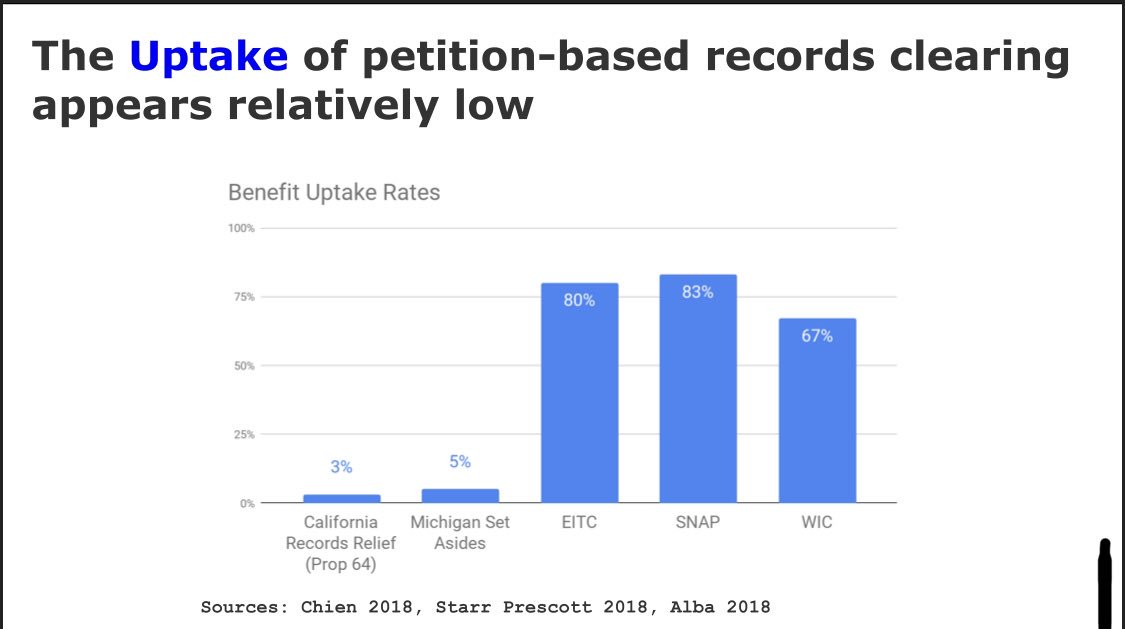
\includegraphics[width=\textwidth]{images/chien-via-twitter.jpeg}
    \caption{Take-up of record sealing (via Twitter)}
    \label{fig:chien-via-twitter}
\end{figure}

\end{document}

%
% Please see the package documentation for more information
% on the APA6 document class:
%
% http://www.ctan.org/pkg/apa6
%